
\subsection{Klassen und ihre Funktionen}
\begin{wrapfigure}{l}{0.7\textwidth}
	\vspace{-20pt}
	\begin{center}
		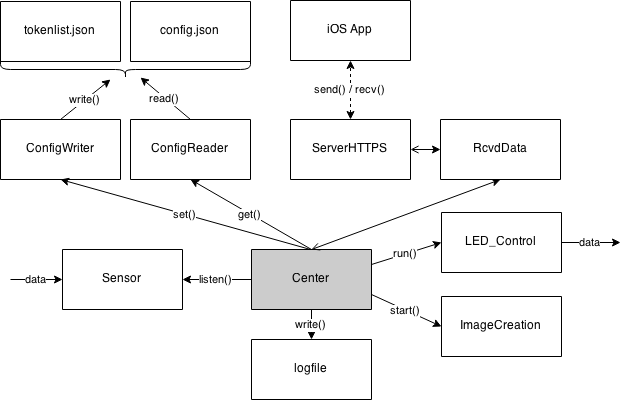
\includegraphics[width=0.7\textwidth]{./data/ApplicationConcept.png}
	\end{center}
	\vspace{-20pt}
	\caption{Anwendungskonzept}
	\vspace{-10pt}
\end{wrapfigure}
Die Klasse 'Center' stellt die zentrale Stelle in der Anwendung dar, an der alle Informationen zusammen laufen und verwaltet werden. In der Klasse 'Sensor' werden die einzelnen Bewegungssensoren überwacht. Falls eine Bewegung detektiert wird, so werden in 'Center' die notwendigen Methoden aufgerufen um die LEDs an- oder auszuschalten.\\\\
Die Klasse 'LED\_Control' verwaltet die eingerichteten LEDs und steuert diese. Hier werden auch die möglichen Effekte gesteuert. Die Methoden in dieser Klasse werden aus der Klasse 'Center' aufgerufen. Ein Zugriff in die andere Richtung ist nicht möglich. \\\\
Alle Serverfunktionaltitäten werden in der Klasse 'Server' bereitgestellt. Hier werden die Daten von Übertragungen empfangen und ausgewertet. Die Prüfung der Korrektheit der einzelnen Protokollbestandteile findet ebenfalls hier statt. Wenn alle Überprüfungen erfolgreich sind, werden die Befehle an 'Center' weiter gegeben und dort ausgeführt. Wenn eine Antwort notwendig ist, zum Beispiel eine Statusabfrage der App an den Server, so werden die Informationen von 'Center' gesammelt und dann von 'Server' verpackt und in korrektem Format an das Mobilgerät gesendet. \\\\
Informationen die für den Betrieb des Systems notwendig sind, werden in der 'Config.ini' gespeichert und können nur über die Klasse 'ConfigReader' abgerufen werden. Es werden Informationen wie Anzahl der LEDs, Passworthash oder Adresse der Netzwerkkamera abgespeichert. Die Konfigurationsdatei wird beim Installationsvorgang erstellt. \\\\
Abrufen von Bildmaterial von der Netzwerkkamera findet ausschließlich über die Klasse 'Cam' statt. Die Klasse ruft die Informationen ab und filtert das Bildmaterial. Somit geben die Methoden der Klasse nur ein Bild zurück. \\\\
In der Klasse 'Status' kann ein Status des Gesamtsystems in der Kommandozeile ausgegeben werden und über 'Log' können Informationen im Logfile gespeichert werden. \\\\
Einzelne Rückgabetypen von Methoden, sowie die Initialisierung von allen Klassen kann mit 'UNIT\_Test' getestet werden. \\\\

\begin{lstlisting}[caption=Ausgabe der Klasse UNIT\_Test, language=python, frame=single, breaklines=true,columns=fullflexible, commentstyle=\color{gray}\upshape, captionpos=b, numbers = left]
root@raspberrypi:/home/timo/Studienarbeit# python UNIT_Test.py 
test_Center (__main__.TestSequenceFunctions) ... ok
test_Effects (__main__.TestSequenceFunctions) ... ok
test_LEDControl (__main__.TestSequenceFunctions) ... ok
test_Sensor (__main__.TestSequenceFunctions) ... ok
test_Server (__main__.TestSequenceFunctions) ... ok
test_Status (__main__.TestSequenceFunctions) ... ok
test_camAdress_MUST_FAIL (__main__.TestSequenceFunctions) ... FAIL
test_camAvaible (__main__.TestSequenceFunctions) ... ok
test_getHashPass (__main__.TestSequenceFunctions) ... ok
test_getMotionPin1 (__main__.TestSequenceFunctions) ... ok
test_getNumberOfLED (__main__.TestSequenceFunctions) ... ok

=============================================
FAIL: test_camAdress_MUST_FAIL (__main__.TestSequenceFunctions)
--------------------------------------------
Traceback (most recent call last):
  File "UNIT_Test.py", line 67, in test_camAdress_MUST_FAIL
    self.assertEqual(resultTest, resultCorrect)
AssertionError: '192.168.2.205' != '123'

--------------------------------------------
Ran 11 tests in 1.873s
\end{lstlisting}
\subsection{Threads}

\begin{wrapfigure}{l}{0.4\textwidth}
	\vspace{-20pt}
	\begin{center}
		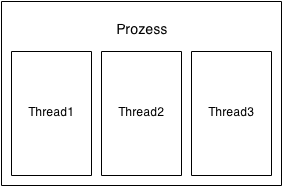
\includegraphics[width=0.3\textwidth]{./data/Threads.png}
	\end{center}
	\vspace{-20pt}
	\caption{Prozess und Threads}
	\vspace{-10pt}
\end{wrapfigure}

\paragraph{Problem:} \\ Die Server-Klasse und Sensor-Klasse befinden sich in einer Endlosschleife, da sie dauerhaft auf eine Eingabe warten. Beim Server sind dies Empfangene Daten und beim Sensor Bewegungssignale. Würden alle Klassen in einem Thread ablaufen, so würde nur eine Klasse gestartet werden und der Anwendungsablauf in dieser bleiben. 
\paragraph{Lösung:} \\ Die beiden oben genannten Klassen, sowie weitere Klassen wie die LED-Steuerung, werden in eigene Threads ausgelagert. Threads sind Unterprozesse im Hauptprozess, die es ermöglichen mehrere Aufgaben in einem Programm gleichzeitig abzuarbeiten. Zwischen den einzelnen Threads kann Datenaustausch statt finden und es ist möglich übergreifende Funktionen aufzurufen. \\
Zur Implementierung wird das Modul 'threading' genutzt. Eine Klasse, die in einem Thread gestartet werden soll, benötigt eine init- und eine run-Methode.
\paragraph{Beispielcode:}\\
Für eine FUnktionsdarstellung der Threads mit Python werden drei Klassen angelegt, eine zur Steuerung und zwei, die in einem Thread laufen sollen. \\
Die Klasse 'Testcenter' initialisiert die Klassen als Threads und startet diese.
\begin{lstlisting}[caption=Klasse Testcenter, language=python, frame=single, breaklines=true,columns=fullflexible, commentstyle=\color{gray}\upshape, captionpos=b, numbers = left]
#!/usr/bin/python
# -*- coding: utf-8 -*-
##############################
# Author: Timo Höting                        #
# Mail: mail[at]timohoeting.de            #
##############################
import threading
from TestThread import *
from TestThread1 import *

class TestCenter():
    def newThread(self):
        global testthread
        global testthread1
        testthread = TestThread('thread0', self)
        testthread1 = TestThread1('thread1', self)
        testthread.start()
        testthread1.start()

    def dosth(self):
        print 'dosth'

    def dosth2(self):
        print 'dosth2'

    def dosth3(self):
        testthread1.calledFromMain('-dosth3')

if __name__ == "__main__":
    newThread = TestCenter()
    newThread.newThread()
\end{lstlisting}
Die beiden TestThread-Klassen enthalten beide eine init- und eine run-Methode. Die Klasse Thread1 enthält zusätzlich noch eine Methode die von anderen Klassen ausführbar ist. 
\begin{lstlisting}[caption=Klasse TestThread1, language=python, frame=single, breaklines=true,columns=fullflexible, commentstyle=\color{gray}\upshape, captionpos=b, numbers = left]
#!/usr/bin/python
# -*- coding: utf-8 -*-
##############################
# Author: Timo Höting                        #
# Mail: mail[at]timohoeting.de            #
##############################

import threading
import time
import datetime

class TestThread1(threading.Thread):
    def __init__(self,ms,c):
        threading.Thread.__init__(self)
        global center
        center = c
        global message
        message = ms

    def run(self):
        print message
        center.dosth2()

    def calledFromMain(self, message):
        print  'calledFromMain' + message
\end{lstlisting}
Die init-Methoden werden bei der Erzeugung des Threads aufgerufen und die run-Methode wenn er gestartet wird. Danach können die Methoden wie bei normalen Methodenaufrufen benutzt werden. 